\chapter{随机变量}

\begin{introduction}
    \item 离散与连续随机变量
    \item 一元与多元
    \item cdf, pmf, pdf
    \item 条件分布
    \item 独立随机变量
    \item 随机变量函数的分布
    \item 次序随机变量
\end{introduction}

在概率论中,主要关心$X$取值于数值集合$\mathcal{X}$中某个子集$B$的可能性, 即希望得到$\P(\{\omega\in\Omega : X(\omega) \in B\})$. 概率论不关心具体的样本点$\omega\in\Omega$, 将其记为$\{X \in B\} = X^{-1}(B)$. 由于$\P$定义在$\mathscr{F}$上, 故需$X^{-1}(B) \in \mathscr{F}$.

\begin{definition}[可测性]
    设所有值得关心的$B\subset \mathcal{X}$组成$\mathscr{F}_{\mathcal{X}}$, 且$\forall B \in \mathscr{F}_{\mathcal{X}}$都满足$\{X\in B\} \in \mathscr{F}$, 则称$X$为$\mathscr{F}/\mathscr{F}_{\mathcal{X}}$\textbf{可测的}. 当$\mathscr{F}_{\mathcal{X}}$不引起混淆时, 简记为关于$\mathscr{F}$\textbf{可测}, 写作$X \in \mathscr{F}$.
\end{definition}

由于原像保持交、并、补等集合运算, 且$\mathscr{F}$是$\sigma$代数, 可将$\mathscr{F}_{\mathcal{X}}$扩张为合适的最小的$\sigma$代数, 即$\sigma(\mathscr{F}_{\mathcal{X}})$, 因此可测映射的定义不妨\underline{只考虑$\mathscr{F}_{\mathcal{X}}$是$\sigma$代数}的情况.

\begin{definition}[随机变量]
    为了表示因随机性而变动的量, 称\underline{可测映射}(measurable mapping)
    \[ X : (\Omega,\mathscr{F},\P) \to (\mathcal{X},\mathscr{F}_{\mathcal{X}}), \quad \omega\in\Omega \mapsto X(\omega)\in\mathcal{X} \]
    为\textbf{随机元}(random element), 也称\textbf{随机变量}(random variable). 其中$\mathscr{F}_{\mathcal{X}}$
\end{definition}

由于只考虑$\mathscr{F}_{\mathcal{X}}$是$\sigma$代数的情况, 可将随机变量看作将原概率空间映射到新概率空间的方式. 新样本空间由\underline{Borel点集}构成, 对应的概率测度等于原像的.

\begin{remark}
    使用随机变量$X$时, 有两个可能的含义:
    \begin{itemize}
        \item $X$的(随机)取值
        \item $X$的分布
    \end{itemize}
\end{remark}

\begin{definition}[离散与连续随机变量]
    当$\mathcal{X}$是 (至多可数的) 离散点集, $\mathscr{F}_{\mathcal{X}}$由$\mathcal{X}$的所有子集组成, 则称其为\textbf{离散随机变量}(discrete random varible). 当随机变量$\mathcal{X} = \R^{n}$, 考虑$\mathscr{F}_{\mathcal{X}}$为$\left\{\prod_{i=1}^{n}(-\infty,x_{i}] : x_{1},\dots,x_{n}\in\R\right\}$生成的Borel代数(最小的$\sigma$代数), 则称其为\textbf{连续随机变量}(continuous random varible).
\end{definition}

\section{随机变量的分布}

\begin{definition}
    称随机元$X$诱导的\underline{概率测度}
    \[ \P\{X\in\bullet\},\ \bullet\in\mathscr{F}_{\mathcal{X}} \]
    为$X$的\textbf{概率分布}(distribution/law)
\end{definition}
\begin{remark}
    对于随机变量, 他的取值是随机的, 但他的分布是固定的
\end{remark}

\begin{definition}[单变量分布函数]
    一个函数$F : \R \to [0,1]$称为一个单变量分布函数,当其满足以下性质时:
    \begin{description}
        \item[单调性] $F(x_1)\le F(x_2) , \quad \forall x_1<x_2$
        \item[右连续性] $\lim_{x \to x_0^+}F(x)=F(x_0)$
        \item[有界性] $\lim_{n \to -\infty}F(x)=0, \quad \lim_{n \to \infty}F(x)=1$
    \end{description}
\end{definition}

\begin{property}
    $F(x)$最多只有可数个间断点
\end{property}

\begin{proposition}
    对每个分布$Q: \mathscr{B}_1 \to [0,1]$都存在唯一一个分布函数$F_Q : \R \to [0,1]$使得$F_Q(x)=Q[(-\infty,x]], \quad \forall x \in \R$成立。
\end{proposition}

\begin{proposition}
    对每个分布函数$F : \R \to [0,1]$都存在唯一一个分布$Q_F: \mathscr{B}_1 \to [0,1]$使得$Q_F[(-\infty,x]]=F(x), \quad \forall x \in \R$成立。
\end{proposition}

\begin{theorem}
    分布函数可以唯一决定概率分布, 即:
    \[ Q_{F_Q}=Q, \quad F_{Q_F}=F \]
    把随机变量$X$服从分布函数$F(x)$简记作$X \thicksim F(x)$
\end{theorem}

\begin{table}[h]
    \centering
    \begin{tabular}{|c|cc|}
        \hline
                                      & \multicolumn{1}{c|}{离散}                                 & 连续                        \\ \hline
        \multirow{3}{*}{一元随机变量} & \multicolumn{1}{c|}{概率质量函数(pmf)}                    & 概率密度函数(pdf)           \\ \cline{2-3}
                                      & \multicolumn{2}{c|}{累积分布函数(cdf)}                                                  \\ \cline{2-3}
                                      & \multicolumn{2}{c|}{矩母函数/特征函数(mgf/chf)}                                         \\ \hline
        \multirow{3}{*}{多元随机变量} & \multicolumn{1}{c|}{联合概率质量函数(joint pmf)}          & 联合概率密度函数(joint pdf) \\ \cline{2-3}
                                      & \multicolumn{2}{c|}{联合累积分布函数(joint cdf)}                                        \\ \cline{2-3}
                                      & \multicolumn{2}{c|}{联合矩母函数/特征函数(joint mgf/chf)}                               \\ \hline
    \end{tabular}
\end{table}

\begin{definition}[累积分布函数]
    此时$X = (X_{1},\dots,X_{n})^{\top}$的分布由(累积)\textbf{分布函数}(cumulative distribution function, c.d.f.)
    \[ F_{X}(x_{1},\dots,x_{n}) = \P\{X_{1}\leq x_{1},\dots, X_{n}\leq x_{n}\}, \quad x_{1},\dots,x_{n}\in\R. \]
    唯一刻画. 把随机变量$X$服从分布函数$F(x)$简记作$X \thicksim F(x)$
\end{definition}

\begin{figure}[h]
    \centering
    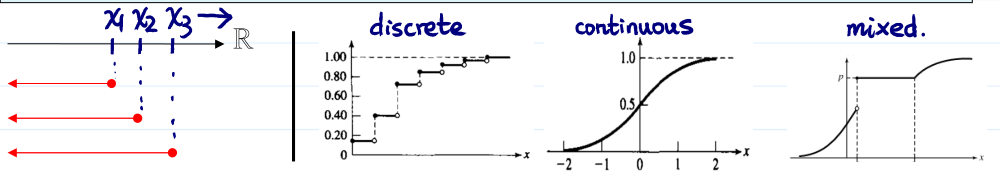
\includegraphics[width=0.8\textwidth]{image/cdf.png}
\end{figure}

\begin{definition}[概率质量函数]
    当且仅当函数$p(x)$满足下述条件时, 被称为\textbf{概率质量函数}(probability mass function, p.m.f.):
    \begin{itemize}
        \item $p(x)\ge 0$
        \item $\sum_{x \in \X}p(x)=1$
    \end{itemize}
\end{definition}

当$X$是离散型随机变量, 设$\mathscr{F}_{\mathcal{X}}$由$\mathcal{X}$的所有子集组成, 此时$X$的分布由
\[ p_{X}(x) = \P\{X=x\} = \P(\{\omega\in\Omega:X(\omega)=x\}), \quad x\in\mathcal{X} \]
唯一刻画. 其与分布函数间的关系为:
\begin{itemize}
    \item $F(x) = \sum_{t\le x}P(X=t)=\sum_{t\le x}p(t)$
    \item $p(x)=P(X=x)=F(x)-F(x-)$
\end{itemize}

\begin{definition}[概率密度函数]
    当且仅当函数$f(x)$满足下述条件时, 被称为\textbf{概率密度函数}(probability density function, p.d.f.):
    \begin{itemize}
        \item $f(x)\ge 0$
        \item $\int_{-\infty}^{\infty}f(x)=1$
    \end{itemize}
\end{definition}

当$X$是连续型随机变量, 且$F_{X} : \R^{n} \to [0,1]$可微(或者更一般地, \underline{绝对连续}), 此时$X$的分布由
\[ f_{X} := \frac{\partial^{n} F_{X}}{\partial x_{1} \cdots \partial x_{n}} \]
唯一刻画. 其与分布函数间的关系为:
\begin{itemize}
    \item $F(x) = \int_{-\infty}^x f(t)dt$
    \item $f(x)=\frac{d}{dx}F(x)$
\end{itemize}

\begin{remark}
    即使对于$f(x)>0$的$x$, $P(X=x)=x\int_{x}^x f(t)dt=0$, 即连续型随机变量在实轴上任意一点的概率测度为零. 概率密度函数$f(x)$代表的是在此位置上单位长度的概率, 可能是一个很大的值.
\end{remark}

\section{多元随机变量}

\begin{definition}[随机向量]
    若随机变量$X_1(\omega), X_2(\omega),\cdots , X_n(\omega)$定义在\underline{同一概率空间}$(\Omega,\mathscr{F},\P)$上, 则称
    \[ X(\omega) = (X_1(\omega), X_2(\omega),\cdots , X_n(\omega)) \]
    构成一个n维\textbf{随机向量},亦称n维随机变量.
\end{definition}

\begin{proposition}
    若$B_n$为$\R^n$上任一博雷尔点集,有
    \[ \{ X(\omega) \in B_n \} \in \mathscr{F} \]
\end{proposition}

\begin{definition}
    称n元函数
    \[ F(x_1,x_2, \cdots , X_n)=\P \{ X_1(\omega)<x_1, X_2(\omega)<x_2,\cdots , X_n(\omega)<x_n \} \]
    为随机向量$X(\omega)$的\textbf{联合分布函数}(joint cdf).
\end{definition}

当$n=2$时,有
\begin{equation}\label{equ:2dim_Prob}
\P((a_1,b_1)\le X < (a_2,b_2))=F(b_1,b_2)-F(a_1,b_2)-F(b_1,a_2)+F(a_1,a_2)
\end{equation}

\begin{property}
    多元分布函数的一些性质:
    \begin{enumerate}
        \item 单调性:关千每个变元是单调不减函数;
        \item \begin{align*}
                  F(x_1,x_2, \cdots, -\infty, \cdots, X_n)=0 \\
                  F(+\infty,+\infty, \cdots, , +\infty)=1
              \end{align*}
        \item 关于每个变元右连续.
        \item 在二元场合,还应该有:对任意$ a_1 <b,,a_2<b_2$ ,都有
              \[ F(b_1,b_2)-F(a_1,b_2)-F(b_1,a_2)+F(a_1,a_2)\ge 0   \]
    \end{enumerate}
\end{property}

为保证\ref{equ:2dim_Prob}式中的概率的非负性,性质4是必须的,而且由性质4可以推出单调性,但存在着反例说明,由单调性并不能保证性质4的成立(见习题 12) .这是多元场合与一元场合的不同之处.

\subsection{边际分布}

\begin{definition}
    对于多维随机变量$X$, 只考虑其中一个分量的分布时, 称其为$X$的\textbf{边际分布或边缘分布}. 对于分量$X_i$, 其\textbf{边缘分布函数}(marginal cdf)为:
    \[ F_{X_i}(x_i) = \P\{ X_i \le x_i \} = F(\infty,\cdots , x_i ,\cdots ,\infty)\] 
\end{definition}



\subsection{独立}

\begin{definition}[独立随机变量]
    若随机变量$X(\omega) = (X_1(\omega), X_2(\omega),\cdots , X_n(\omega))$联合分布函数可分解成各分量边缘分布函数的乘积, 即:
    \[ F(x_1,x_2,\cdots ,x_n) = F_{X_1}(x_1)F_{X_2}(x_2)\cdots F_{X_n}(x_n) , \quad \forall x_1,x_2,\cdots ,x_n \in \R \] 
    则称随机变量$X$各分量相互\textbf{独立}
\end{definition}

\begin{remark}
    对于一般的多元随机变量, 其各分量边缘分布不足以描述联合分布的情况. 但若其各分量独立则可以.
\end{remark}

\begin{theorem}
    对于连续情况:
    \begin{align*}
        &F(x_1,x_2,\cdots ,x_n) = F_{X_1}(x_1)F_{X_2}(x_2)\cdots F_{X_n}(x_n) \\
        \Leftrightarrow & f(x_1,x_2,\cdots ,x_n) = f_{X_1}(x_1)f_{X_2}(x_2)\cdots f_{X_n}(x_n)
    \end{align*}
    对于离散情况:
    \begin{align*}
        &F(x_1,x_2,\cdots ,x_n) = F_{X_1}(x_1)F_{X_2}(x_2)\cdots F_{X_n}(x_n) \\
        \Leftrightarrow & p(x_1,x_2,\cdots ,x_n) = p_{X_1}(x_1)p_{X_2}(x_2)\cdots p_{X_n}(x_n)
    \end{align*}
\end{theorem}

\begin{theorem}
    若随机变量$X,Y$独立, 则其变换$Z=g(X), W=h(Y)$也独立.

    泛化情况:若随机向量$\{X\}_n$各分类独立, 则其变换$\{Y\}_n=g(\{X\}_n)$各分类也独立.
\end{theorem}

\subsection{条件分布}

\begin{definition}
	对一切使 $P\left(Y=y_{j}\right)=p_{ \cdot j}=\sum_{i=1}^{+\infty} p_{i j}>0$ 的 $y_j$, 称
	\begin{equation}\label{eq:3.5.1}
		p_{i | j}=P\left(X=x_{i} | Y=y_{j}\right)=\frac{P\left(X=x_{i}, Y=y_{j}\right)}{P\left(Y=y_{j}\right)}
		=\frac{p_{i j}}{p_{\cdot j}}, \quad i=1,2, \ldots
	\end{equation}
	为给定 $Y=y_j$ 条件下 $X$ 的条件分布列. 若$p_X(x)=0$, 则定义其为0.
\end{definition}

设二维连续随机变量 $(X,Y)$ 的联合密度函数为 $p(x,y)$, 边际密度函数为 $p_X(x),p_Y(y)$.

在离散随机变量场合, 其条件分布函数为 $P(X\leq x|Y=y)$. 但是, 因为连续随机变量取某个值的概率为零, 即 $P(Y=y)=0$, 所以无法用条件概率直接计算 $P(X\leq x|Y=y)$, 一个很自然的想法是: 将 $P(X\leq x|Y=y)$ 看成是 $h\to 0$ 时 $P(X\leq x|y\leq Y\leq y+h)$ 的极限, 即
\begin{align*}
	P(X \leq  x | Y=y) & =\lim _{h \to 0} P(X \leq  x | y \leq  Y \leq  y+h)                                                          \\
	                   & =\lim _{h \to 0} \frac{P(X \leq  x, y \leq  Y \leq  y+h)}{P(y \leq  Y \leq  y+h)}                            \\
	                   & =\lim _{h \to 0} \frac{\int_{-\infty}^{x} \int_{y}^{y+h} p(u, v) dv du}{\int_{y}^{y+h} p_{Y}(v) dv} \\
	                   & =\lim _{h \to 0} \frac{\int_{-\infty}^{x} \left\{ \frac{1}{h} \int_{y}^{y+h} p(u, v) dv \right\} du}
	{\frac{1}{h} \int_{y}^{y+h} p_{Y}(v) dv}.
\end{align*}
当 $p_Y(y),p(x,y)$ 在 $y$ 处连续时, 由积分中值定理可得
\begin{align*}
	 & \lim _{h \to 0} \frac{1}{h} \int_{y}^{y+h} p_{Y}(v) dv=p_{Y}(y), \\
	 & \lim _{h \to 0} \frac{1}{h} \int_{y}^{y+h} p(u, v) dv=p(u, y).
\end{align*}
所以
\[
	P(X \leq x | Y=y)=\int_{-\infty}^{x} \frac{p(u, y)}{p_{Y}(y)} du.
\]
至此, 我们可以定义连续随机变量的条件分布如下.

\begin{definition}
	对一切使 $p_Y(y)>0$ 的 $y$, 给定 $Y=y$ 条件下 $X$ 的\textbf{条件分布函数}\index{T!条件分布函数}和
	\textbf{条件密度函数}\index{T!条件密度函数}分别为
	\begin{align}
		 & F(x | y)=\int_{-\infty}^{x} \frac{p(u, y)}{p_{Y}(y)} du,  \\
		 & p(x | y)=\frac{p(x, y)}{p_{Y}(y)}.
	\end{align}
	同理对一切使 $p_Y(y)>0$ 的 $x$, 给定 $X=x$ 条件下 $Y$ 的条件分布函数和条件密度函数分别为
	\begin{align}
		 & F(y | x)=\int_{-\infty}^{y} \frac{p(x, v)}{p_{X}(x)} dv  \\
		 & p(y | x)=\frac{p(x, y)}{p_{X}(x)}.
	\end{align}
\end{definition}

\begin{remark}
    对于每一个\underline{固定的$x$}, $p_{Y|X}(y|x)$是一个关于$y$的概率质量函数; $f_{Y|X}(y|x)$是一个关于$y$的概率密度函数
\end{remark}

与概率三定理的对应:
\begin{description}
    \item[乘法法则] $p_{XY}(x,y)=p_{Y|X}(y|x)p_{X}(x), \quad f_{XY}(x,y)=f_{Y|X}(y|x)f_{X}(x)$
    \item[全概率公式] $p_{Y}(y)=\sum_{x}p_{Y|X}(y|x)p_{X}(x), \quad f_{Y}(y)=\int^{+\infty}_{-\infty}f_{Y|X}(y|x)f_{X}(x)dx$
    \item[Bayes原理]  $p_{X|Y}(x|y)=\frac{p_{Y|X}(y|x)p_{X}(x)}{\sum_{x}p_{Y|X}(y|x)p_{X}(x)}, \quad f_{X|Y}(x|y)=\frac{f_{Y|X}(y|x)f_{X}(x)}{\int^{+\infty}_{-\infty}f_{Y|X}(y|x)f_{X}(x)dx}$
\end{description}

\section{随机变量的函数}

